\documentclass[10pt,a4paper]{article}
\usepackage[utf8]{inputenc}
\usepackage{amsmath}
\usepackage{amsfonts}
\usepackage{amssymb}
%\usepackage[outputdir=build]{minted}
\usepackage[]{minted}
\usepackage{hyperref}
\usepackage{makecell}
\usepackage{color,soul}
\renewcommand\theadfont{\bfseries}
\usepackage[color=blue!10,textsize=footnotesize,textwidth=25mm]{todonotes}
\author{Dan Printzell}
\title{GSOC 2019 Proposal \\
Replace Runtime Hooks with Templates}
\begin{document}

\maketitle


\begin{center}
\begin{tabular}{ r | l }
\href{mailto:gsoc@vild.io}{gsoc@vild.io} & \url{https://vild.io/} \\
FreeNode: Wild & \url{https://github.com/Vild} \\
\end{tabular}
\end{center}

\normalsize\textbf{Contact}

\begin{tabular}{ l l }
Address: & 
\begin{tabular}{l}
Dan Printzell \\
\hl{Address} \\
\hl{Address2} \\
Sweden 
\end{tabular} \\
Phone number: & \hl{Phone number} \\
\end{tabular}

\normalsize\textbf{Emergency contact - \hl{Who?}}

\begin{tabular}{ l l }
Address: & 
\begin{tabular}{l}
\hl{Name} \\
\hl{Address} \\
\hl{Address2} \\
Sweden 
\end{tabular} \\
Phone number: & \hl{Phone number}\\3
Email: & \href{mailto:nobody@example.com}{\hl{Email}} \\
\end{tabular}

\section{Problem Introduction}
Runtime hooks are an important part of the D ecosystem as they allow the 
compiler to express complicated operations with the help of a function call. Sadly, some of
the current runtime hooks present safety concerns, as Mike Franklin explains in 
the \textit{[gsoc] DMD - Ideas} thread \cite{DMDIdeas} that when writing
\mintinline{d}{array.length = 8;} - which is lowered to 
\mintinline{d}{_d_arraysetlengthT} - it is allowed in a \mintinline{d}{@safe 
pure nothrow} scope, even if this expression is
lowered to a function that is not \mintinline{d}{@safe pure nothrow}. Lucia 
Cojocarus\cite{GenericLightweightRuntime} brought forward another problem, explaining that some of these runtime
hooks add a lot of indirection, which in turn adds to execution time overhead.

The solution to fix these issues is to change the runtime hooks to use templates 
instead of the \mintinline{d}{TypeInfo} class hierarchy. This solution was 
presented by both Cojocarus and Franklin, and it solves the safety issue as the 
implementation can be resolved at compile time rather than trust that the 
runtime developer will correctly implement the hooks. Additionally, the 
indirection is also solved as the hook can access the real type directly and use 
Design by Introspection techniques to further optimize the code for the 
specified type. Furthermore, by changing the hooks to use templates it will make 
it easier to get contributions as the code is now located only in the runtime 
instead of both the runtime and the compiler\cite[at 00:04:45]{GenericLightweightRuntime}. The conversion will also help with 
goal of turning the runtime into a \textit{pay for what you use} library.

The expected outcome of this proposal is that all of the array hooks listed in 
Appendix A will be successfully converted into templates.

\section{Why me}
I have been programming for over 10 years now, and I am currently studying for a 
master’s degree in computer science at BTH in Sweden. I found D in early 2014 
and have been using it since in a variety of hobby projects; as well as a few 
school assignments. Additionally, I’m one of the volunteers that maintains the D 
packages on Arch Linux\cite{TrustedUsers} and I operate a Discord server\footnote{D Language Code Club - \url{https://discord.gg/bMZk9Q4}} around the D language with 
other like-minded fanatics.

The biggest D project I’m working on is PowerNex\footnote{An operating system written in D - \url{https://github.com/PowerNex/PowerNex}}, a from-scratch operating 
system I have been the sole developer of for more than three and a half years. 
It is this project that has taught me the most about runtime hooks, as before 
the existence of betterC PowerNex used a bare-metal runtime written by Adam D. 
Ruppe\cite{MinimalZip}. I was lucky to get this base code from Ruppe as it helped start the 
PowerNex project. As the D language evolved it required more and more new hooks 
to accommodate the growing set of runtime features, thus requiring me to learn 
and implement them to use the newer versions of D.

PowerNex has taught me how to traverse DMD’s source code I needed to write 
patches\footnote{PowerNex patches for dmd - \url{https://github.com/PowerNex/powernex-dmd}} to compile code for the PowerNex target instead on any of the other 
backend targets. These patches had to touch the frontend, to define 
\mintinline{d}{version=PowerNex} instead of \mintinline{d}{version=linux}, and 
the backend, to output a correct PowerNex executables.

The reasons for applying to GSoC and for wanting to work on this task is because 
I have felt for a long time that I want to help with the development of the 
language, but because I am a full time student I have not had the time to do any 
contributions. With the help of GSoC I can make this dream come true as I can 
make sure that my bills will be paid whilst helping the D language evolve.

\section{Method}
The steps for doing the conversion are based on the suggestions made by Mike 
Franklin in the \textit{[GSoC] Trying to find a good topic} newsgroup thread\cite{Suggestions} and 
from Lucia Cojocarus talk\cite{GenericLightweightRuntime}. 

\textbf{Convert hook.}  There is many tasks that need to be done to complete the 
conversion to a template. These include changing all the references to 
\mintinline{d}{TypeInfo} to use the type directly, changing allocation methods 
to use match the safety requirements, replacing input data checks with their 
template counterparts, and fixing all the problems that shows up during the 
conversion. The next step is to add unittest to test that this template works 
like its non-template counterpart.

\textbf{Compiler support.} The task here is to make the compiler instantiate the 
new template instead of calling the old hook. It is important to add unittests 
here as well to ensure it will not break any code.

The druntime and the compiler PRs will be worked on the same time to be able to 
catch both compiler and runtime problems. One problem that could happen is that 
the CTFE get triggers and throws a error. This needs to be fixed before any of 
the PR have been submitted. After verifying that everything works as expected, 
and it will not break any code, the changes can be submitted as a PR to druntime 
and a PR to dmd. The dmd PR requires that the druntime PR has already been 
merged to not break any of the automated testers or anyone compiling a nightly 
build of the compiler. Along with the PR benchmark results will be submitted. 
These results give a quick overview of how important the change is for the 
language and incase of a performance degradation, if the hook needs to be 
changed in the near future.

\textbf{Clean up.} The last task after all PRs have been merged, is to submit a 
cleanup PR to druntime that removes the old, and now unused, hook.

There are a few places where problem could halt or slow down the developments. 
There are of course bugs that need to be fixed, but these bugs will only be 
fixed if they are caused by the translation phase, if the bugs are from the old 
hook they should be fixed in a separate PR. This is to ensure that the code 
review on the PR should be as smooth and fast as possible and throwing in more 
changes than needed could be detrimental to the review process.

Another problem could happy would be that during the code review improvements 
could be suggested on how the translation could be done. This problem should be 
expected and planned for so it does not negatively influence the schedule.


\section{Expected outcome}
The expected outcome of this problem would be that all of the array hooks will 
be have been translate to templates. There will not be any expectation that 
these hooks will work in betterC mode. It would be a plus but it is not an 
expected outcome. There is a possibility that bugs will be found during the 
conversion and these will be reported to the bugtracker. Fixing these inside the 
PR will make the PR harder to review and fixing the bugs may break code.

\section{Timeline}
This is a rough estimate of how the time plan will look like. If a hook is 
easier than expected and I finish early I will continue with the hooks for the 
week after. If I run out of array hooks to convert I will contact my supervisor 
to try and find more hooks that I could convert.
My goal is to work at least 30 hours a week, which breaks down to six hour per 
day, five days per week, but I will probably work more than than that. The only
time where I might not be able to work fulltime is week 22 - 23 as these are the
last weeks of school and I will have two exams. To make sure that this does not
hurt the GSoC I have put a bit less work these weeks compared to the rest.

The metric used to plan which symbols to do each week is the lines of code 
inside each hook. This values should show a \textit{in-a-ballpark} how hard it 
will be to translate the hook. Hooks that have a lot in common like all the 
different versions of \mintinline{d}{_d_arrayappend} will be translated at the 
same time. All the hooks on their own can be seen in Appendix \ref{appendix:hooks}
and a visualization of the lines of code per week can be seen in Appendix \ref{appendix:timelinegraph}.

\begin{center}
\begin{tabular}{| l | p{6cm} | l |}
\hline
\thead{Date} & \thead{Goal} & \thead{Lines of code} \\ \hline
May 27 & \textbf{Start of GSoC} & \\  \hline
W.22 - W.23 & \_d\_arrayappend* & 144 \\ \hline
W.24 - W.25 & \makecell[l]{\_d\_arraysetctor\\\_d\_arrayctor\\\_d\_arraycat*} & 190 \\ \hline

June 24 - 28 & \textbf{First evaluation} & \\ \hline
W.26 - W.27 & \_d\_arraysetlength* & 432 \\ \hline
W.28 - W.29 & \makecell[l]{\_d\_arrayliteral*\\\_d\_arraysetcapacity} & 202 \\ \hline

July 22 - 26 & \textbf{Second evaluation} & \\ \hline
W.30 - W.31 & \makecell[l]{\_d\_delarray\_t*\\\_d\_arrayassign*\\\_d\_arrayshrinkfit\\\_d\_arraysetassign} & 174 \\ \hline
W.32 - W.33 & \_d\_newarray* & 183 \\ \hline
August 19 - 26 & \textbf{Last evaluation} & \\ \hline
\end{tabular}
\end{center}

\newpage
\bibliography{proposal.bib}
\bibliographystyle{ieeetr}

\appendix
\section{Appendix A - Hooks to be translated}
\label{appendix:hooks}
These hooks where found by running:
\definecolor{bg}{rgb}{0.95,0.95,0.95}
\small
\begin{minted}[breaklines,breakanywhere,bgcolor=bg]{bash}
egrep -o -R "_d_.*array.*\(.*[^;]$" | grep -v "assocarray" | grep "TypeInfo"
\end{minted}

\small
\begin{minted}[breaklines]{text}
Module: rt.arrayassign
    _d_arrayassign, Lines: 16
    _d_arrayassign_l, Lines: 36
    _d_arrayassign_r, Lines: 20
    _d_arrayctor, Lines: 32
    _d_arraysetassign, Lines: 22
    _d_arraysetctor, Lines: 28
Module: rt.lifetime
    _d_arrayshrinkfit, Lines: 41
    _d_arraysetcapacity, Lines: 168
    _d_newarrayU, Lines: 55
    _d_newarrayT, Lines: 11
    _d_newarrayiT, Lines: 29
    _d_newarraymTX, Lines: 11
    _d_newarraymiTX, Lines: 11
    _d_delarray_t, Lines: 25
    _d_arraysetlengthT, Lines: 192
    _d_arraysetlengthiT, Lines: 208
    _d_arrayappendT, Lines: 13
    _d_arrayappendcTX, Lines: 99
    _d_arraycatT, Lines: 61
    _d_arraycatnTX, Lines: 35
    _d_arrayliteralTX, Lines: 19
Module: rt.tracegc
    _d_newarrayTTrace, Lines: 15
    _d_newarrayiTTrace, Lines: 15
    _d_newarraymTXTrace, Lines: 18
    _d_newarraymiTXTrace, Lines: 18
    _d_delarray_tTrace, Lines: 14
    _d_arrayliteralTXTrace, Lines: 15
    _d_arraycatTTrace, Lines: 16
    _d_arraycatnTXTrace, Lines: 18
    _d_arrayappendTTrace, Lines: 16
    _d_arrayappendcTXTrace, Lines: 16
    _d_arraysetlengthTTrace, Lines: 16
    _d_arraysetlengthiTTrace, Lines: 16
\end{minted}

\section{Appendix B - Timeline graph}
\label{appendix:timelinegraph}
\begin{center}
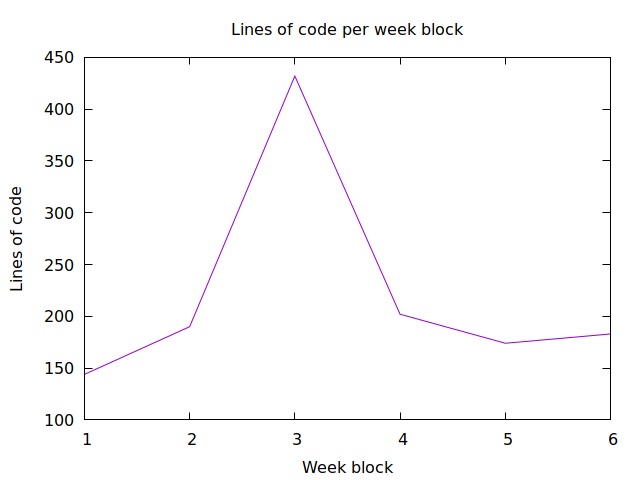
\includegraphics[height=8cm]{WeekValue}
\end{center}

\end{document}